\newpage
\section{Problem Formulation}
\label{section:problem}

Please present the formulation in this section. You may want to cover the following aspects:

\begin{itemize}
    \item Your notations (e.g. MDPs, value functions, function approximators,...etc)
    \item The optimization problem of interest
    \item The technical assumptions
\end{itemize}

\subsection{Preliminaries and Notations}

\begin{figure}[htb]
    \center
    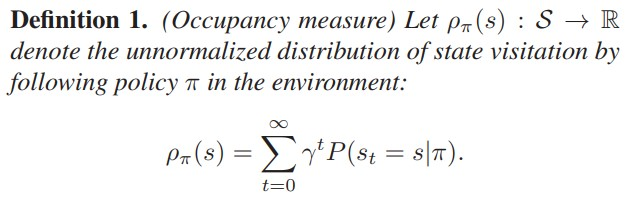
\includegraphics[width=10cm]
    {def1}
    \label{fig: def1}
\end{figure} 

From the Def. 1, for better exploiting demonstrations, this research first converts the expected discounted reward from Eq. (1) to a Eq. (2) defined on occupancy measure (Ho Ermon, 2016). 

\begin{figure}[htb]
    \center
    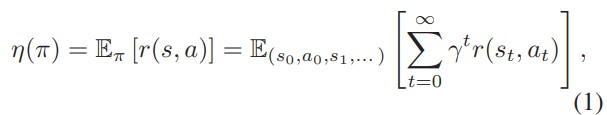
\includegraphics[width=9cm]
    {eq1}
    \label{fig: eq1}
\end{figure} 

\begin{figure}[htb]
    \center
    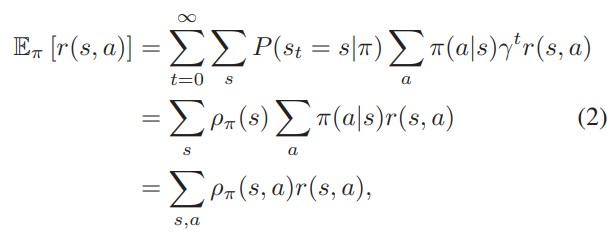
\includegraphics[width=9cm]
    {eq2}
    \label{fig: eq2}
\end{figure} 

In the following lemma (\cite{syed2008game}), the occupancy measure has an important property that it uniquely specifies a policy. 

\begin{figure}[h!]
    \center
    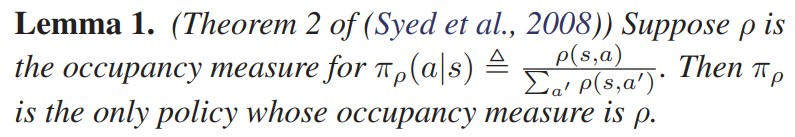
\includegraphics[width=10cm]
    {lemma1}
    \label{fig: lemma1}
\end{figure} 

Besides, in addition to sparse rewards from environments, the agent is also provided with a few demonstrations $D^{E}=\left\{\tau_{1},\tau_{2},...,\tau_{N}\right\}$, where the $i$-th trajectory $\tau_{i}=\left\{(s^{i}_{0},a^{i}_{0}),(s^{i}_{1},a^{i}_{1}),...,(s^{i}_{T},a^{i}_{T}) \right\}$ is generated from executing an unknown expert policy $\pi_{E}$.


\subsection{The optimization problem of interest}

Besides maximizing the expected return $\eta(\pi_{\theta})$ through learning from sparse feedback, this research also encourages the agent to explore by “following” the demonstrations DE. Then an introduce demonstration-guided exploration term $L_{M}(\pi_{\theta},\pi_{E})=D_{JS}(\pi_{\theta},\pi_{E})$ is introduced to the vanilla objective $\eta(\pi_{\theta})$. This gives a new learning objective:

\begin{figure}[h!]
    \center
    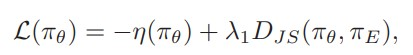
\includegraphics[width=6.5cm]
    {eq3-0}
    \label{fig: eq3-0}
\end{figure} 

Where $\lambda_{1}$ is a trading-off parameter, and $D_{JS}$ is the Jensen-Shannon divergence between current policy $\pi_{theta}$ and the expert one $\pi_{E}$. However, this divergence measure is infeasible since $\pi_{E}$ is unknown. Instead, we redefine the divergence over the occupancy measures $\rho_{\pi}(s,a)$ and $\rho_{\pi_{E}}(s,a)$ by Lemma 1. And finally the proposed demonstration guided learning objective is changed to the Eq. (3)

\begin{figure}[h!]
    \center
    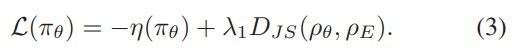
\includegraphics[width=7cm]
    {eq3}
    \label{fig: eq3}
\end{figure} 


\subsection{The technical assumptions}

Although the expert policy may not best one, but its quality is usually better than the agent policy in early training stage. Therefore, this paper presents a reasonable and necessary assumption, and it will be used to prove the benefits of exploration with demonstrations.

\begin{figure}[h!]
    \center
    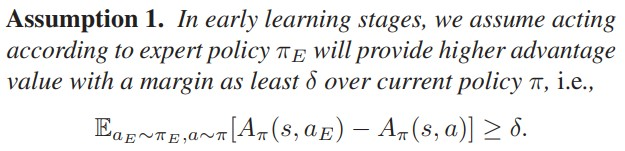
\includegraphics[width=10cm]
    {assump1}
    \label{fig: assump1}
\end{figure} 

And the second assumption is the same when using the form of surrogate objective when proving the TRPO algorithm (\cite{schulman2015trust}).

\begin{figure}[h!]
    \center
    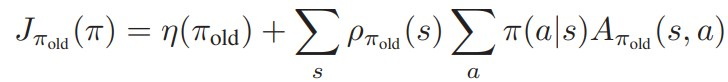
\includegraphics[width=9cm]
    {eq5-1}
    \label{fig: eq5-1}
\end{figure}


The assumption is, the reason why $\rho_{\pi}$ is replaced by $\rho_{\pi_{old}}$ is that the change in state distribution can be ignored due to policy update.